\documentclass[lesson_slides]{subfiles}
\usepackage{graphicx}
% \graphicspath{ {./images/} }
\usepackage{enumerate}
\usepackage{pifont} % for ding
\usepackage{float} % keeps tables in the exact position they occupy in the code
\usepackage{gb4e} % leave last



\begin{document}
%%=-=-=-=-=-=-=-=-=-=-=-=-=-=-=-=-=-=-=-=-=-=-=-=-=-=-=-=-=-=-=-=-=-=-=-=-=-=-=-=
%   FRAME START   -=-=-=-=-=-=-=-=-=-=-=-=-=-=-=-=-=-=-=-=-=-=-=-=-=-=-=-=-=-=-=
\begin{frame}[c]{What's a parameter?}

    \transboxin<1>
    \transglitter<2>
    \transwipe<3>
    \textbf{\textsc{parameter}} (Rizzi 2017: 165) \pause
    
    'an instruction for the triggering of a syntactic operation, expressed as a morphosyntactic feature
associated to a functional head'.

\end{frame}
%   FRAME END   --==-=-=-=-=-=-=-=-=-=-=-=-=-=-=-=-=-=-=-=-=-=-=-=-=-=-=-=-=-=-=
%=-=-=-=-=-=-=-=-=-=-=-=-=-=-=-=-=-=-=-=-=-=-=-=-=-=-=-=-=-=-=-=-=-=-=-=-=-=-=-=
%   FRAME START   -=-=-=-=-=-=-=-=-=-=-=-=-=-=-=-=-=-=-=-=-=-=-=-=-=-=-=-=-=-=-=
\begin{frame}[c]{Syntactic operations}

    \transboxin<1>
    \transglitter<2>
    \transwipe<3>
    \noindent\textbf{\textsc{syntactic operations}} \pause
    \begin{itemize}
        \item[\ding{227}] simple; \pause
        \item[\ding{227}] highly learnable; \pause
        \item[\ding{227}] restricted to an extremely reduced set for reasons of learnability.
    \end{itemize}	
    
\end{frame}
%   FRAME END   --==-=-=-=-=-=-=-=-=-=-=-=-=-=-=-=-=-=-=-=-=-=-=-=-=-=-=-=-=-=-=
%=-=-=-=-=-=-=-=-=-=-=-=-=-=-=-=-=-=-=-=-=-=-=-=-=-=-=-=-=-=-=-=-=-=-=-=-=-=-=-=
%   FRAME START   -=-=-=-=-=-=-=-=-=-=-=-=-=-=-=-=-=-=-=-=-=-=-=-=-=-=-=-=-=-=-=
\begin{frame}[c]{Syntactic operations (ii)}

    \transboxin<1>
    \transglitter<2>
    \transwipe<3>
    \noindent\textbf{\textsc{available syntactic operations}} \pause
        \begin{xlist}
            \ex Merge \pause
            \ex Move \pause
            \ex Spellout
        \end{xlist}
\end{frame}
%   FRAME END   --==-=-=-=-=-=-=-=-=-=-=-=-=-=-=-=-=-=-=-=-=-=-=-=-=-=-=-=-=-=-=

%   FRAME START   -=-=-=-=-=-=-=-=-=-=-=-=-=-=-=-=-=-=-=-=-=-=-=-=-=-=-=-=-=-=-=
\begin{frame}[c]{Move}

    \transboxin<1>
    \transglitter<2>
    \transwipe<3>
    \noindent\textbf{\textsc{move}} \pause
    \begin{itemize}
        \item[\ding{227}] complex operation (à la \citealt{chomsky2001});\\ \pause
        \item[\ding{227}] involves either a head or a phrase;\\ \pause
        \item[\ding{227}] encompasses the establishment of a probe-goal search followed by (internal) merge of the goal.
    \end{itemize}
        
\end{frame}
%   FRAME END   --==-=-=-=-=-=-=-=-=-=-=-=-=-=-=-=-=-=-=-=-=-=-=-=-=-=-=-=-=-=-=
%=-=-=-=-=-=-=-=-=-=-=-=-=-=-=-=-=-=-=-=-=-=-=-=-=-=-=-=-=-=-=-=-=-=-=-=-=-=-=-=
\begin{frame}[c]{Phrasal movement vs. Head movement}

    \transboxin<1>
    \transglitter<2>
    \transwipe<3>
    \noindent\textbf{\textsc{phrasal movement}} (\citealt{rizzi2017}: 171 (20)) \pause
        \begin{xlist}
            \ex A search feature at the phrasal level. \pause
            \ex The corresponding internal merge feature at the phrasal level (IM) ('EPP feature'). \pause
        \end{xlist}

    \noindent\textbf{\textsc{head movement}} (\citealt{rizzi2017}: 171 (21)) \pause
        \begin{xlist}
            \ex A search feature at the lex level (Search\textsubscript{lex} Feature) \pause
            \ex The corresponding internal merge feature, again at the lex level (IM\textsubscript{lex} Feature)
        \end{xlist}
        
\end{frame}

%%%%%%%%%%%%%%%%%%%%
\begin{frame}{Combinations}

    \begin{center}
        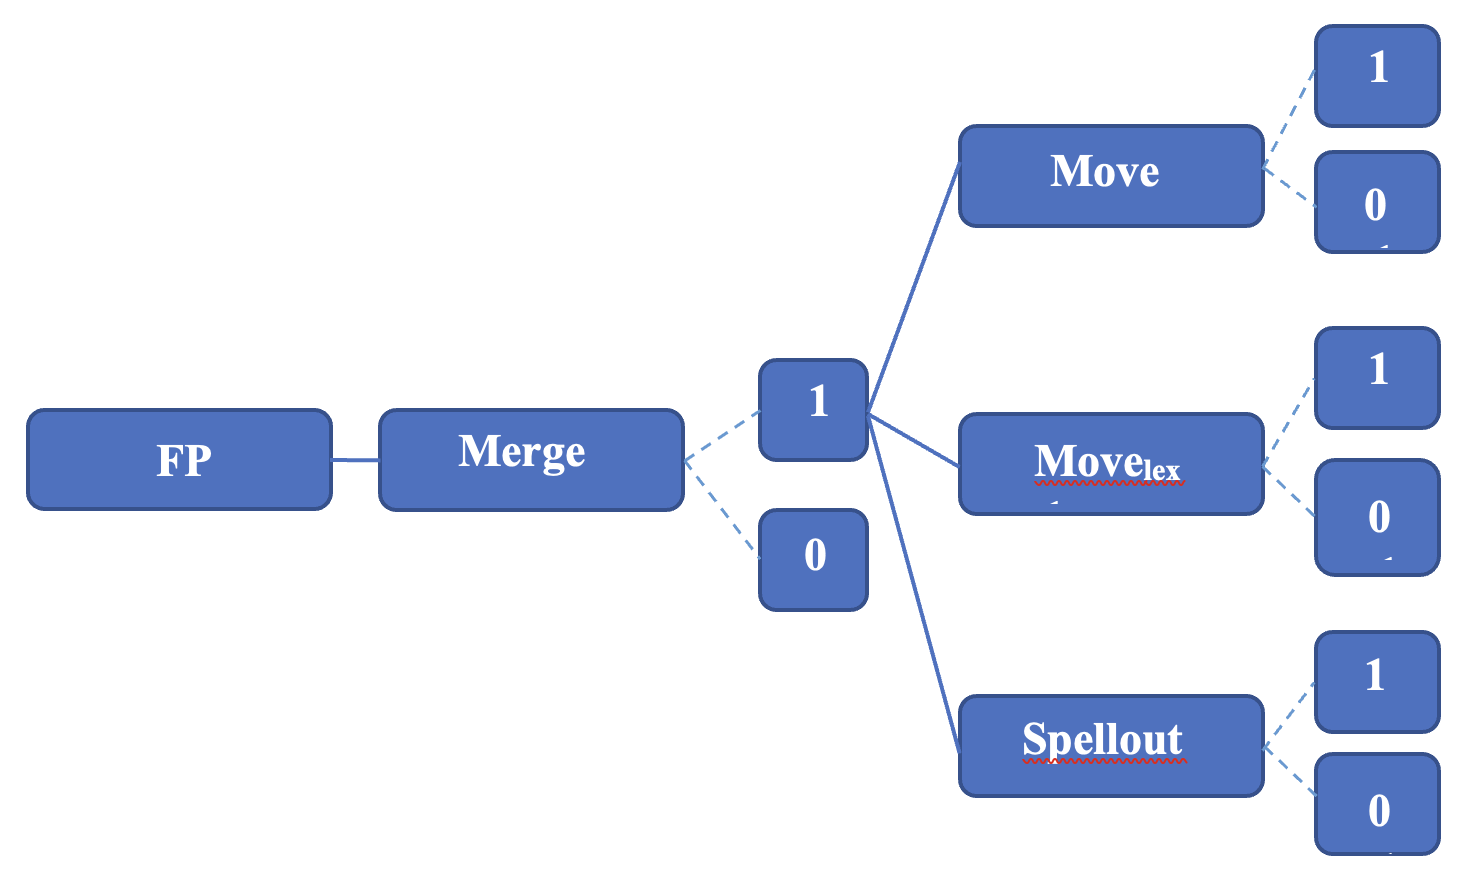
\includegraphics[width=12cm, height=6cm]{images/combinations.png}
    \end{center}
    
\end{frame}
%%%%%%%%%%%%%%%%%%%%
%%%%%%%%%%%%%%%%%%%%
\begin{frame}{Combinations (ii)}

    \begin{table}[H]
        \centering
        \begin{tabular}{|l|r|r|r|r|r|r|r|r|r|}
        \hline
         & I & II & III & IV & V & VI & VII & VIII \\
        \hline
        Move                    & 1 & 1 & 1 & 1 & 0 & 0 & 0 & 0 \\
        \hline
        Move\textsubscript{lex} & 1 & 0 & 0 & 1 & 1 & 0 & 1 & 0 \\
        \hline
        Spellout                & 1 & 0 & 1 & 0 & 1 & 1 & 0 & 0 \\
        \hline
        \end{tabular}
        \caption{\label{tab:samp}Parametric variations: possible combinations.}
    \end{table}
    
\end{frame}
%%%%%%%%%%%%%%%%%%%%
%%%%%%%%%%%%%%%%%%%%
\begin{frame}{Combinations (ii)}

    \begin{table}[H]
        \centering
        \begin{tabular}{|l|r|r|r|r|r|r|r|r|r|}
        \hline
         & I & II & III & IV & V & VI & VII & VIII \\
        \hline
        Move                    & \hl{1} & 1 & 1 & 1 & 0 & 0 & 0 & 0 \\
        \hline
        Move\textsubscript{lex} & \hl{1} & 0 & 0 & 1 & 1 & 0 & 1 & 0 \\
        \hline
        Spellout                & \hl{1} & 0 & 1 & 0 & 1 & 1 & 0 & 0 \\
        \hline
        \end{tabular}
        \caption{\label{tab:samp}Parametric variations: possible combinations.}
    \end{table}
    
\end{frame}
%%%%%%%%%%%%%%%%%%%%
%%%%%%%%%%%%%%%%%%%%
\begin{frame}{Combinations (ii)}

    \begin{table}[H]
        \centering
        \begin{tabular}{|l|r|r|r|r|r|r|r|r|r|}
        \hline
         & I & II & III & IV & V & VI & VII & VIII \\
        \hline
        Move                    & 1 & 1 & 1 & 1 & 0 & 0 & 0 & \hl{0} \\
        \hline
        Move\textsubscript{lex} & 1 & 0 & 0 & 1 & 1 & 0 & 1 & \hl{0} \\
        \hline
        Spellout                & 1 & 0 & 1 & 0 & 1 & 1 & 0 & \hl{0} \\
        \hline
        \end{tabular}
        \caption{\label{tab:samp}Parametric variations: possible combinations.}
    \end{table}
    
\end{frame}
%%%%%%%%%%%%%%%%%%%%
\end{document}